\section{Estensibilità}\label{Estensibilita}

\subsection{Aggiungere un Webhook}

Per aggiungere una nuova tipologia di Webhook parser, è sufficiente estendere l'interfaccia \texttt{Webhook}
e un eventuale \texttt{WebhookFactory} in caso si tratti di una nuova applicazione.

\begin{figure}[H]
    \centering
    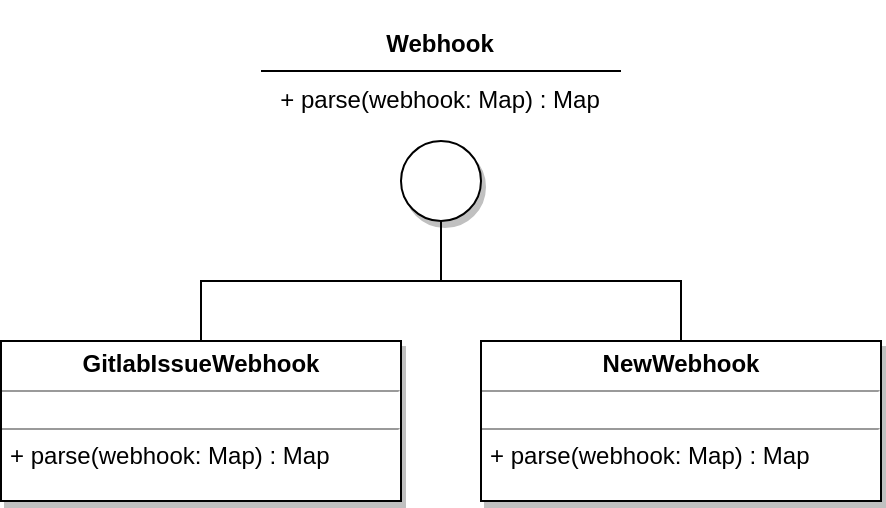
\includegraphics[width=0.7\textwidth]{img/EstensioneWebhook-Webhook.png}\\
    \caption{Aggiungere un Webhook parser}
\end{figure}


\begin{figure}[H]
    \centering
    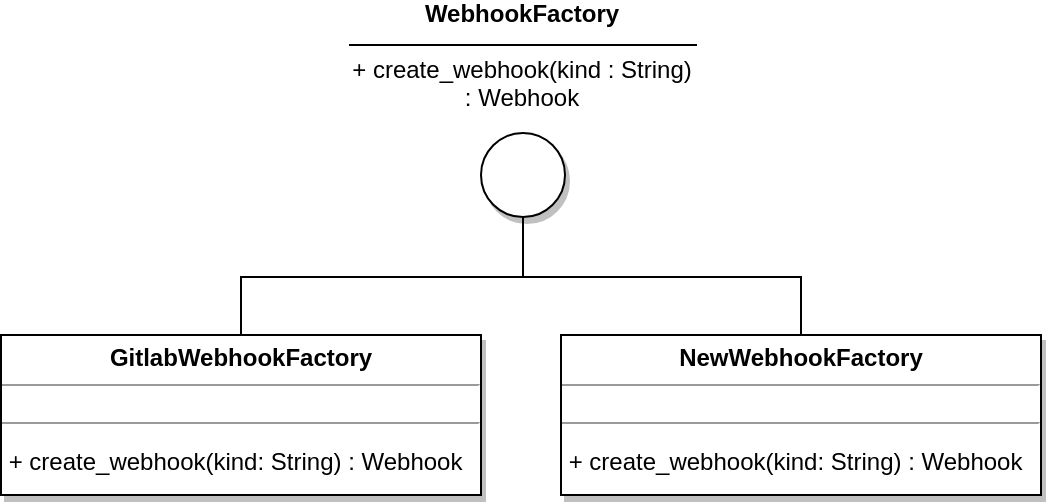
\includegraphics[width=0.7\textwidth]{img/EstensioneWebhook-Factory.png}\\
    \caption{Aggiungere una Factory}
\end{figure}

Se è un nuovo webhook di un'applicativo esistente, è necessario che la factory conosca la tipologia di webhook.
Aggiungere tale informazione al metodo \texttt{create\_webhook(kind)}.


\subsection{Aggiungere un Producer}

Per aggiungere un Producer di una nuova applicazione, creare una nuova classe che estenda la classe astratta \texttt{Producer}.
Definire il metodo astratto \texttt{webhook\_kind(webhook)}.

\begin{figure}[H]
    \centering
    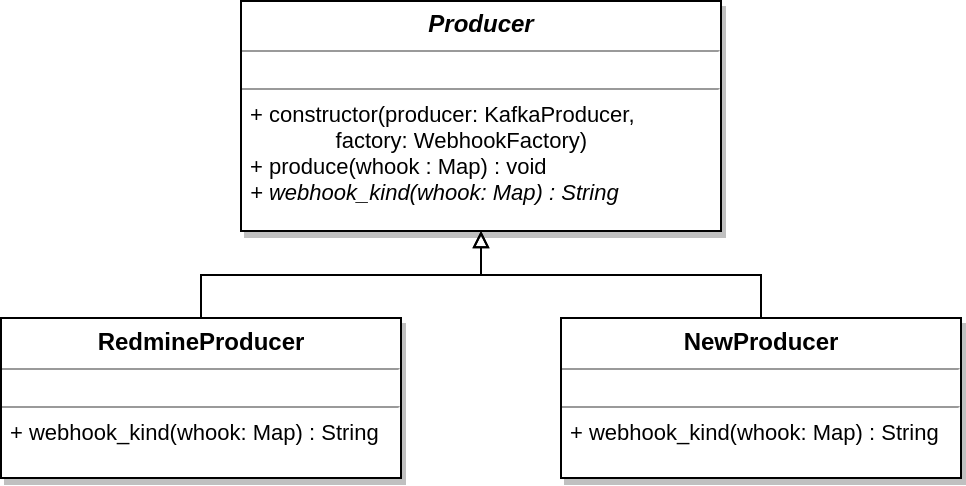
\includegraphics[width=0.7\textwidth]{img/EstensioneProducer.png}\\
    \caption{Aggiungere un Producer}
\end{figure}


\subsection{Aggiungere un Consumer}

Per aggiungere un Consumer di una nuova applicazione, creare una classe che estenda la classe astratta \texttt{Consumer}.
Definire il metodo astratto \texttt{send(receiver: String, msg: Map)} che, dato in input un destinatario e un insieme di coppie
chiave-valore, produca un messaggio formattato e lo invii al destinatario, tramite le API dell'applicazione sulla quale inviare il messaggio.
È consigliato creare un metodo a parte per la formazione del messaggio.

\begin{figure}[H]
    \centering
    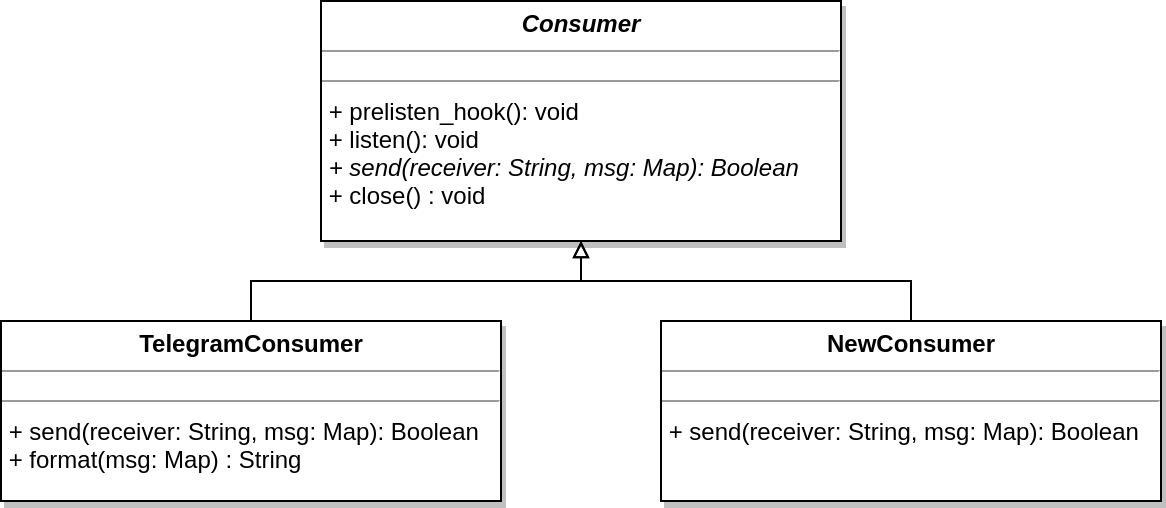
\includegraphics[width=0.7\textwidth]{img/EstensioneConsumer.png}\\
    \caption{Aggiungere un Consumer}
\end{figure}

Viene inoltre offerta la possibilità di ridefinire il metodo \texttt{prelisten\_hook()} che viene chiamato prima che il Consumer si metta effettivamente in ascolto
del topic specifico su Kafka.
È concreto nella class base, ma non fa nulla. Serve per aumentare la flessibilità delle classi che implementano la classe astratta \texttt{Consumer}.


\subsection{Aggiungere un MessageProcessor} \label{EstProcessor}

Per far conoscere al Gestore Personale la presenza di un nuovo tipo di Producer, è necessario creare una classe concreta che erediti da \texttt{Processor} e di conseguenza implementare il metodo \texttt{filter\_users\_by\_topic()}.
Questo perchè ogni tecnologia (come Redmine e Gitlab) può avere un tipo diverso di messaggio da elaborare (una messaggio di issue o un messaggio di push).


\begin{figure}[H]
    \centering
    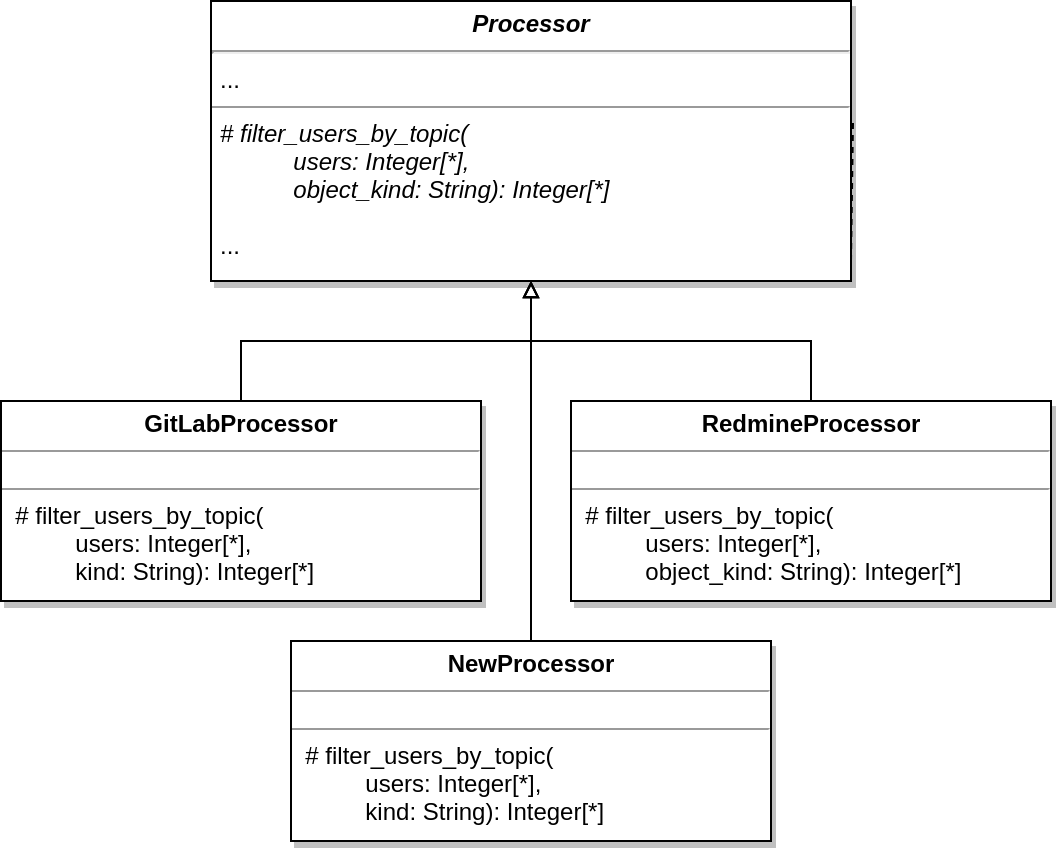
\includegraphics[width=0.7\textwidth]{img/EstensioneGP-Processor.png}\\
    \caption{Aggiungere un Processor}
\end{figure}
